\documentclass[12pt]{article}

\usepackage[spanish]{babel}
\usepackage[utf8x]{inputenc}
\usepackage{amsmath}

\usepackage{hyperref}
\usepackage{url}
\usepackage{gensymb}
\usepackage[dvipsnames]{xcolor}

\usepackage{parskip}
\usepackage{fancyhdr}
\usepackage{multicol}
\usepackage{vmargin}
\usepackage{setspace}
\usepackage{geometry}

\usepackage{float}
\usepackage{array}
\usepackage{graphicx}
\graphicspath{{images/}}
\usepackage{wrapfig}
\usepackage{caption}
\usepackage{subcaption}

\setmarginsrb{2 cm}{1 cm}{2 cm}{1.5 cm}{1 cm}{1 cm}{1 cm}{1 cm}

\title{Determinación del coeficiente de dilatación volumetrica \\ del Agua, Gasolina Magna y Diésel}
\author{Martín Alejandro Paredes Sosa}		

\makeatletter
\let\thetitle\@title
\let\theauthor\@author
\let\thedate\@date										
\makeatother

\pagestyle{fancy}
\fancyhf{}
\rhead{Lic.. Física}
\lhead{Informe 4B}
\cfoot{\thepage}

\begin{document}
%%%%%%%%%%%%%%%%%%%%%%%%%%%%%%%%%%%%%%%%%%%%%%%%%%%%%%%%%%%%%%%%%%%%%%%%%%%%%%%%%%%%%%%%
%\begin{titlepage}
%	\centering
%    \vspace*{0.5 cm}
%    
\includegraphics[scale = 0.5]{logo}\\[0.5 cm]	% University Logo
%    \textsc{\LARGE Universidad de Sonora}\\[1 cm]	% University Name
%	\textsc{\Large División de Ciencias Exactas y Naturales}\\[1 cm]		%		% Course Code
%	\textsc{\large Termodinámica Clásica}\\[0.5 cm]				% Course Name
%	\rule{\linewidth}{0.2 mm} \\[0.4 cm]
\begin{center}
{ \large \bfseries \thetitle}\\
\end{center}
%{ \large \bfseries \thetitle}\\
%	\rule{\linewidth}{0.2 mm} \\[1.25 cm]
%    \textsc{\Large Equipo \#2} \\[1.25 cm]
%\thetitle\\	
	\begin{minipage}{\textwidth}
		\begin{center} 
			%\textsc{\Large Integrantes:} \large \\
			\theauthor 
			\end{center}
	\end{minipage}\\[-0.52 cm]
%===================================================================================================
\begin{abstract}
	Esta experiencia se utilizó el dilatómetro de líquidos, con el cual se midió el cambio en el volumen  conforme se variaba la temperatura a una presión constante. Lo que se busca es que a partir de los cambios del volumen encontrar coeficiente de dilatación volumétrica ($\beta$).

\end{abstract}
\vspace{-1cm}
%===================================================================================================
\section{Introducción}
Esta experiencia en el laboratorio consistió en medir el volumen que ocupa el agua, gasolina y diésel es un dilatómetro de líquidos, el cual se encuentra sumergido en  en una mezcla de agua y etilenglicol colocado en un baño recirculador, en cual se fue aumentando la temperatura. EL objetivo es es encontrar el coeficiente de dilatación volumétrica ($\beta$).

\hspace{0.75cm} Cuando se tiene un solido, liquido o un gas que varia con la temperatura a presión constante es la forma es la que se puede encontrar $\beta$. Su expresión es la siguiente:
\begin{equation}\label{beta}
	\beta = \frac{1}{V} \left(\frac{\partial V}{\partial \theta} \right)_{P}	
\end{equation}
Este valor varia de sustancia a sustancia y esta en función de la temperatura. El valor en sólidos y gases es positivo y en los liquidos la mayor de las veces lo es, excepto en un pequeño intervalo donde este negativo. Un ejemplo de esto es el agua entre 0 y 4 °C.
%===================================================================================================
\section{Desarrollo Experimental}
Para empezar se llenaron tres dilatómetro de 25.5 ml. El dilamómetro consiste en un bulbo de vidrio unido a un capilar graduado y el que se uso tiene una resolución de 0.01 ml. Uno se lleno con agua, otro con diésel y el último con gasolina magna. A estos con una jeringa se les extrajo el exceso para el liquido quedara en la marca de 25.0 ml. 

\hspace{0.75cm} Se fijo la temperatura del reciclador a 20°C. Luego se programo para que la temperatura aumentara a 60°C. Se dejo pasar el tiempo y se tomo dato del volumen y de la temperatura cada que el volumen cambio aproximado de 0.05 ml.
\begin{figure}[H]
\centering
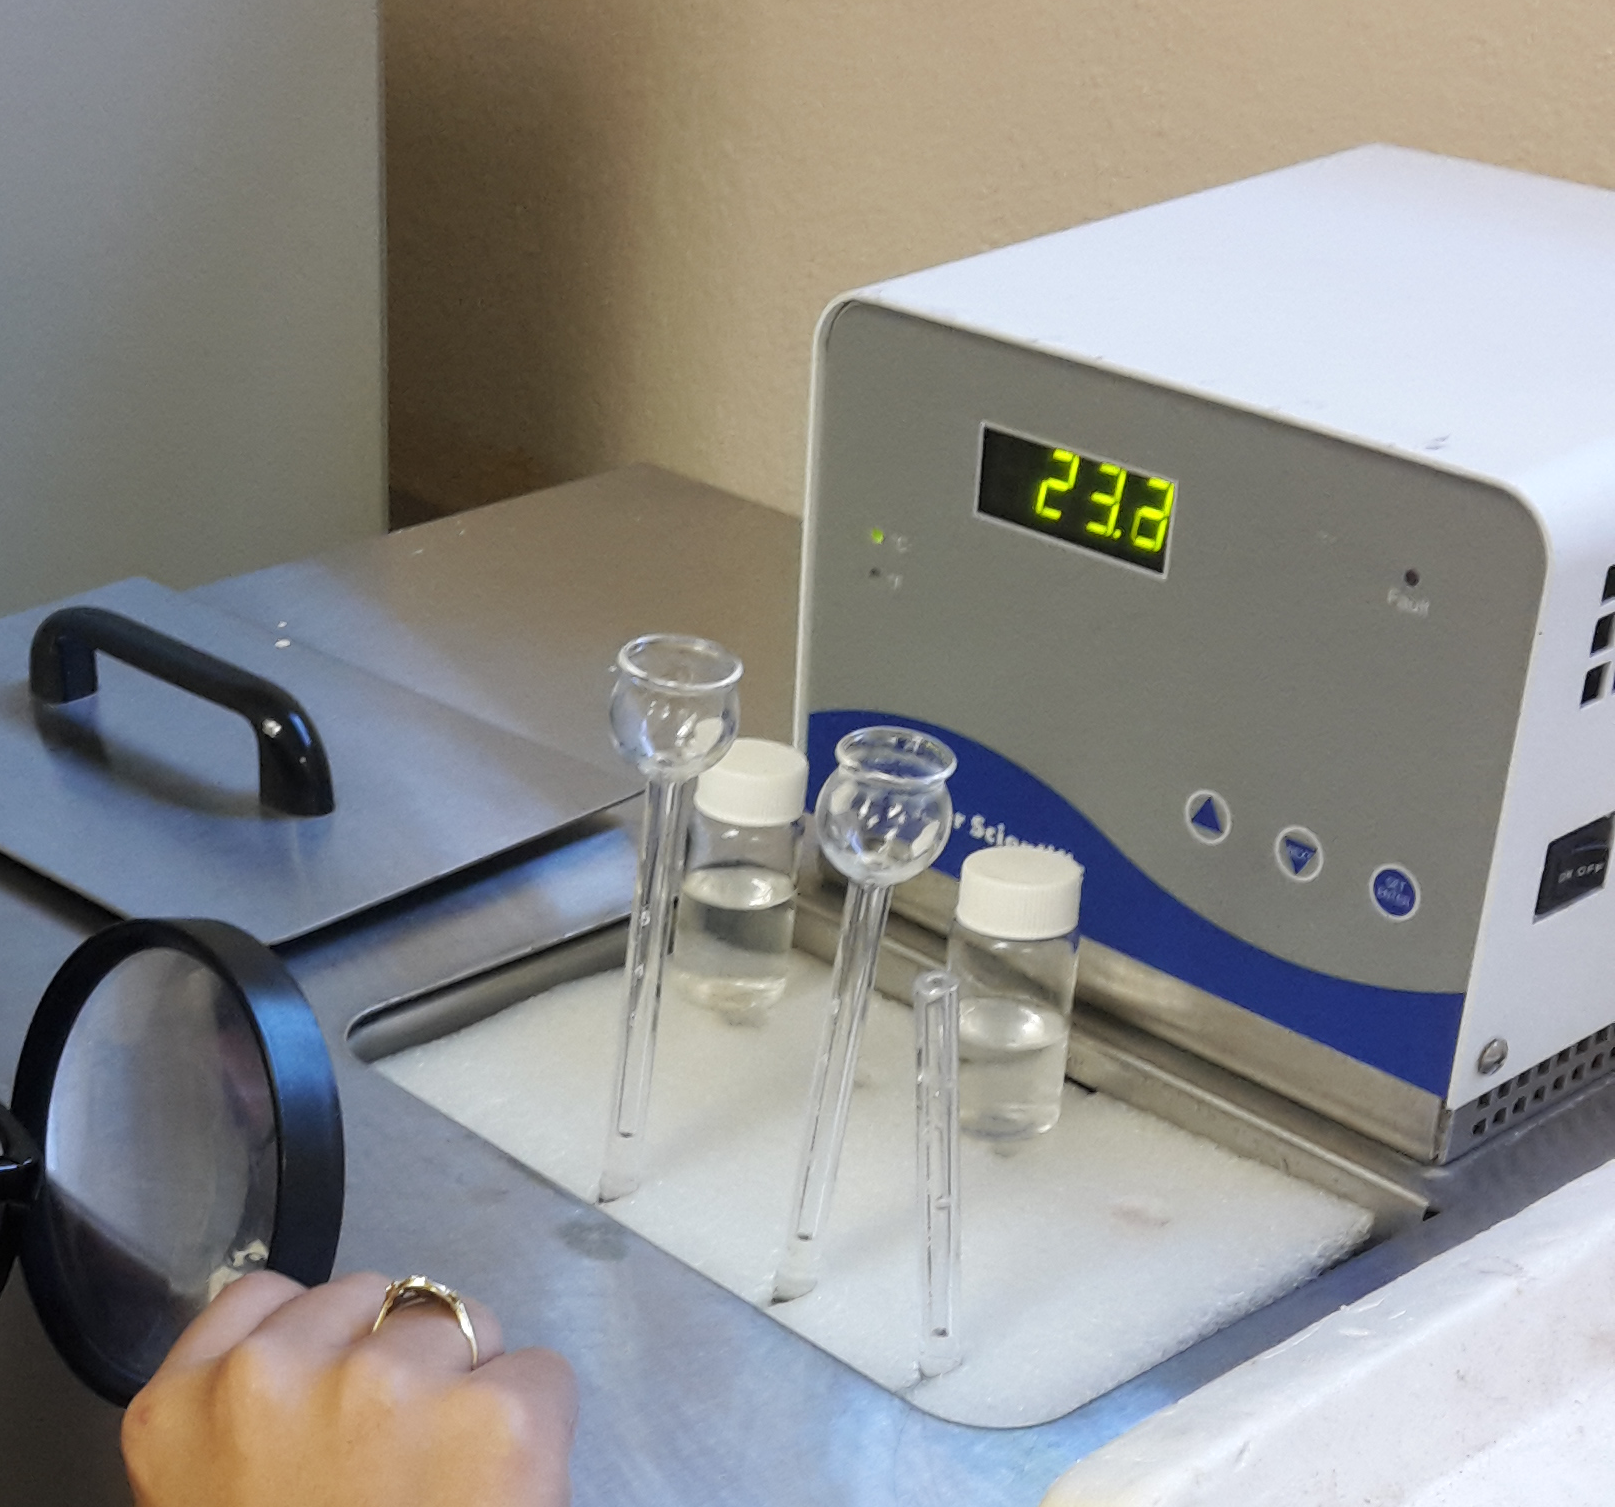
\includegraphics[width=0.25\linewidth]{setup.png}
\caption{Arreglo Experimental}
\end{figure}

Se tuvo cuidado con el diésel y la gasolina ya que estos se podían desbordar.

Para obtener el coeficiente $\beta$ se ocupa realizar modificaciones a \eqref{beta}.
$$\beta = \frac{1}{V} \left(\frac{\partial V}{\partial \theta} \right)_{P}$$


\begin{equation}\label{bet}
\beta = \left(\frac{\partial \ln (V)}{\partial \theta} \right)_{P}
\end{equation}
Para poder aplicar el logaritmo, se tiene que volver adimensional su argumento, por lo que podemos dividir entre su volumen inicial $V_0$) y queda:

\begin{equation}
\beta = \left( \frac{\partial \ln \left(\frac{V}{V_0} \right)  }{\partial \theta} \right) _{P}
\end{equation}


%===================================================================================================
\section{Resultados}
Los valores que se midieron fueron los siguientes:

\begin{table}[H]
\centering
\begin{tabular}{|c|c||c|c||c|c|}
\hline
\multicolumn{2}{|c||}{Diésel}  & \multicolumn{2}{|c||}{Magna}  & \multicolumn{2}{|c|}{Agua} \\ \hline
Volumen (ml) & T° (°C) & Volumen (ml) & T°(°C) &Volumen (ml) & T°(°C) \\\hline
  25.00 $\pm 0.002$ & 20.0$\pm 0.029$& 25.00 $\pm 0.002$ & 20.0$\pm 0.029$ &25.00 $\pm 0.002$ & 20.0$\pm 0.029$ \\\hline
  25.05$\pm 0.002$ & 23.0$\pm 0.029$ & 25.05$\pm 0.002$& 25.5$\pm 0.029$ & 25.05$\pm 0.002$ & 23.2$\pm 0.029$ \\\hline
  25.10$\pm 0.002$ & 25.5$\pm 0.029$ & 25.10$\pm 0.002$& 27.4$\pm 0.029$ & 25.10$\pm 0.002$ & 38.1$\pm 0.029$ \\\hline
  25.15$\pm 0.002$ & 27.4$\pm 0.029$ & 25.15$\pm 0.002$& 30.4$\pm 0.029$ & 25.15$\pm 0.002$ & 44.2$\pm 0.029$\\\hline
  25.20$\pm 0.002$ & 29.7$\pm 0.029$ & 25.20$\pm 0.002$& 32.6$\pm 0.029$ & 25.20$\pm 0.002$ & 48.9$\pm 0.029$\\\hline
  25.25$\pm 0.002$ & 31.0$\pm 0.029$ & 25.25$\pm 0.002$& 35.3$\pm 0.029$ & 25.25$\pm 0.002$ & 54.9$\pm 0.029$\\\hline
  25.30$\pm 0.002$ & 33.0$\pm 0.029$ & 25.30$\pm 0.002$& 38.0$\pm 0.029$ & 25.30$\pm 0.002$ & 58.9$\pm 0.029$\\\hline
  25.35$\pm 0.002$ & 34.9$\pm 0.029$ & 25.35$\pm 0.002$& 40.4$\pm 0.029$ & 25.33$\pm 0.002$ & 60.0$\pm 0.029$\\\hline
  25.40$\pm 0.002$ & 36.6$\pm 0.029$ & 25.40$\pm 0.002$& 42.8$\pm 0.029$ & 25.40$\pm 0.002$ & - \\\hline
  25.45$\pm 0.002$ & 38.4$\pm 0.029$ & 25.45$\pm 0.002$& 45.5$\pm 0.029$ & 25.45$\pm 0.002$ & -\\\hline
  25.50$\pm 0.002$ & 40.5$\pm 0.029$ & 25.50$\pm 0.002$& 48.2$\pm 0.029$ & 25.50$\pm 0.002$ & -\\\hline
\end{tabular}
\caption{Medición de Volumen y Temperatura del los líquidos}
\end{table}
Se puede ver que en el caso del agua se ocupa aumentar aun mas la temperatura para alcanzar los 25.5 ml y que los casos de los combustibles no se ocupa aumentar mucho la temperatura para que este aumente su volumen.
\pagebreak

\hspace{0.75cm} Para encontrar $\beta$ se ocupa observar el comportamiento del  $\ln \left(\frac{V}{V_0} \right)$ con respecto a la temperatura. Los siguientes figuras muestran dicho comportamiento.

\begin{figure}[H]
\centering
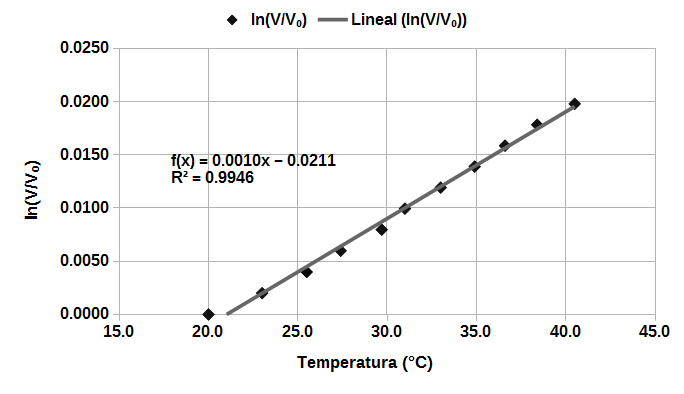
\includegraphics[width=0.5\linewidth]{Diesel.png}
\caption{$\ln \left(\frac{V}{V_0} \right)$ vs T° del Diésel}
\end{figure}
A partir de los datos del Diésel, se le realizó un ajuste lineal.
\begin{equation}
\left(\ln \left(\frac{V}{V_0} \right) \right)_{\theta} = 0.0010 (°C) - 0.0211; \hspace{1.5cm} R^2 = 0.9946
\end{equation}
Es decir, beta seria:
$$\beta_{D} = 0.0010 (°C) $$
\begin{figure}[H]
\centering
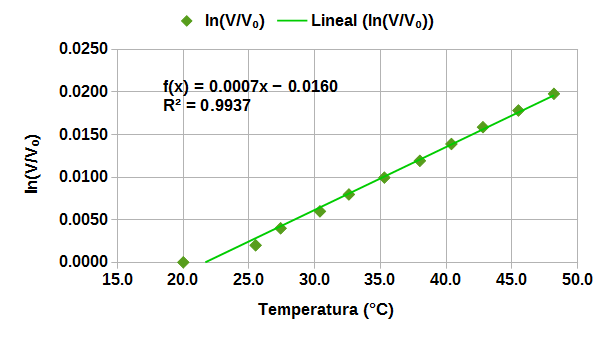
\includegraphics[width=0.5\linewidth]{Magna.png}
\caption{$\ln \left(\frac{V}{V_0} \right)$ vs T° del Magna}
\end{figure}

A partir de los datos del Magna, se le realizó un ajuste lineal.
\begin{equation}
\left(\ln \left(\frac{V}{V_0} \right) \right)_{\theta} = 0.0007 (°C) - 0.0088; \hspace{1.5cm} R^2 = 0.9187
\end{equation}
Es decir, beta seria:
$$\beta_{M} = 0.0007 (°C) $$

\begin{figure}[H]
\centering
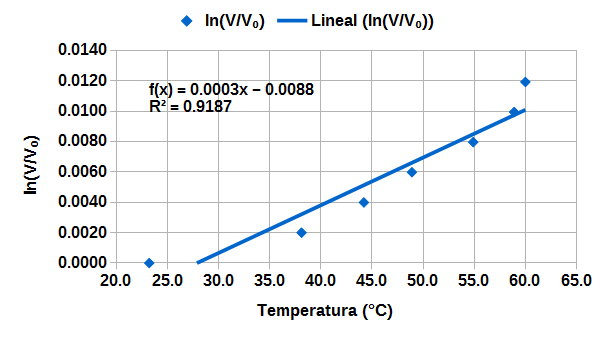
\includegraphics[width=0.5\linewidth]{Agua.png}
\caption{$\ln \left(\frac{V}{V_0} \right)$ vs T° del Agua}
\end{figure}

A partir de los datos del Agua, se le realizó un ajuste lineal.
\begin{equation}
\left(\ln \left(\frac{V}{V_0} \right) \right)_{\theta} = 0.0003 (°C) - 0.0088; \hspace{1.5cm} R^2 = 0.9187
\end{equation}
Es decir, beta seria:
$$\beta_{A} = 0.0003 (°C) $$



\pagebreak


%===================================================================================================
\section{Discusión}
Si modelamos al aire como gas ideal, su ecuación de estado es $PV=nR\theta$.
$$\beta = \frac{1}{V} \left( \frac{\partial V}{\partial \theta} \right) _{P}
 = \frac{1}{V} \left( \frac{\partial \frac{nR\theta}{P})}{\partial \theta} \right) _{P} = \frac{1}{\theta}$$
Por lo que kappa en el gas ideal tiene comportamiento de hipérbola, mientras que el que se obtuvo es una función lineal. Se puede decir que en las condiciones en la que se encontraban estos liquidos no comparten el comportamiento de un gas ideal.
%===================================================================================================
\section{Conclusiones}
Se puede concluir que los resultados que se obtuvieron, pudieran ser mejorados si se hubieran tomado datos en intervalos mas cortos, además de que se vio la relación que existe entre el volumen y la temperatura.

%================================================================================================


\begin{thebibliography}{6}
\bibitem{a}
	Rodríguez Mellado, J.M. (s.f.) \textit{Coeficientes de dilatación térmica y de compresibilidad isotérmico} Recuperado el 19 de Febrero 2017 de	\url{http://www.uco.es/~qf1romej/termodinamica/docs/alfaykappa.pdf}
\bibitem{acu}
Acu\~na, H. (2015). \textit{Manual de Guías de Experiencias en el Laboratorio de Termodinámica Clásica}.

\end{thebibliography}
%================================================================================================

\end{document}

